% article draft @ https://www.overleaf.com/11039646jmkfnhxvqpfp
\documentclass[oneside,12pt]{article}
\usepackage[a5paper,margin=5mm]{geometry}%,showframe
%\usepackage{showframe}
\usepackage[utf8]{inputenc}
\usepackage{xcolor}
\usepackage[colorlinks,
	linkcolor={red!50!black},citecolor={blue!50!black},urlcolor={blue!80!black}]{hyperref}

%% cross references [hrefs]
\usepackage{caption}
\def\figureautorefname~#1\null{fig.#1}
\newcommand{\email}[1]{$<$\href{#1}{#1}$>$}

%% figures
\usepackage[pdftex]{graphicx}
\newcommand{\fig}[4]{
\begin{figure}[h]
{\centering\noindent\includegraphics[#4]{#1}
\protect\caption{#3}\label{fig:#2}}
\end{figure}
}
\newcommand{\figref}[1]{$[$fig.{\ref{#1}}$]$}

% relative sectioning
\usepackage{ifthen}
\newcounter{secdepth}\setcounter{secdepth}{0}
\newcommand{\secup}{\addtocounter{secdepth}{1}}
\newcommand{\secdown}{\addtocounter{secdepth}{-1}}
\newcommand{\secrel}[1]{
\ifthenelse{\equal{\value{secdepth}}{0}}{\part{#1}}{}
\ifthenelse{\equal{\value{secdepth}}{-1}}{\chapter{#1}}{}
\ifthenelse{\equal{\value{secdepth}}{-2}}{\section{#1}}{}
\ifthenelse{\equal{\value{secdepth}}{-3}}{\subsection{#1}}{}
\ifthenelse{\value{secdepth} < -3}{\subsubsection{#1}}{}
}
\newcommand{\secly}[1]{\section*{#1}\addcontentsline{toc}{section}{#1}}
\newcommand{\subsecly}[1]{\section*{#1}\addcontentsline{toc}{subsection}{#1}}

% misc

\renewcommand{\emph}[1]{\textbf{#1}}

% [nosep] option in lists/enums
\usepackage{enumitem}
% frame box
\usepackage{framed}

%% languages/programs

\newcommand{\prog}[1]{\textit{#1}}
\newcommand{\lang}[1]{$#1$}

\newcommand{\C}[1]{\lang{C_{#1}}}
\newcommand{\cpp}{\lang{C_{+^+}}}

\newcommand{\prolog}{\lang{Prolog}}
\newcommand{\xsb}{\prog{XSB}}

\newcommand{\neo}{\prog{neo4j}}



\title{
Using active hypergraph database\\
as software development approach:\\
\Huge{Graph Driven Programming}}

\author{\small{\copyright\ Dmitry Ponyatov \email{dponyatov@gmail.com}, free researcher, 2017}}

\begin{document}
\maketitle
\tableofcontents

\begin{abstract}\noindent
Software development and program architecture engineering has grows complexity in last decades. The existing zoo of programming languages, para\-digms, hardware platforms and operating systems, combined with the software development market requirements, exceeds the capabilities of a particular individual developer. Thus, it is required to create a powerful tool for compensation of software systems development complexity, that combines design tools, RAD, MDP, simulation debugging, static and dynamic analysis of programs, parallel computing support, and, first of all, an expert system and knowledge bases provides knowledge storage, fuzzy search and inference not only in software engineering, but also in applied fields (mathematics and numerical methods, physics, chemistry, mechanics and structural engineering, CAD, electronics, digital signal processing, business planning, accounting and logistics, task and time management, etc).
\end{abstract}

\secly{Introduction}

Software development and program architecture engineering has grows complexity in last decades. This problem is especially notable in hard real-time control systems applied in safety-critical domains: avionics, aerospace, automobiles, and medicine, and covered by tons of safety reglaments and standards. \cite{book1}

If we look on some random typical software developer vacancies, we see huge amount of conventional requirements on knowledge and skills (emphasized in text), making developer live damn scary: to make yourself promising in your profession, you must spend an everyday self-learning in your work and spare time.


\noindent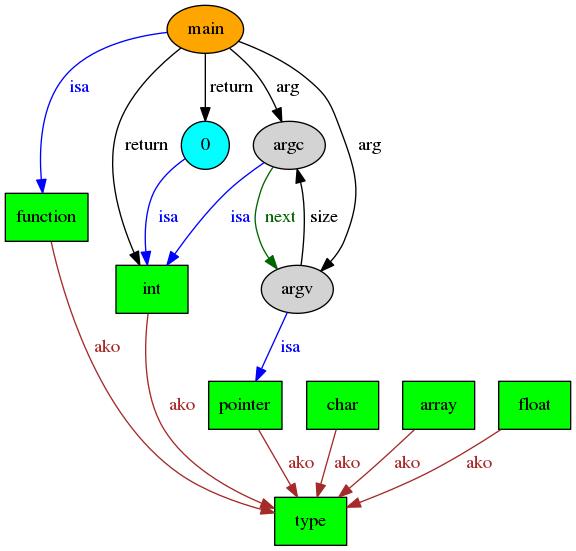
\includegraphics[width=\textwidth]{fig/hello.png}

\noindent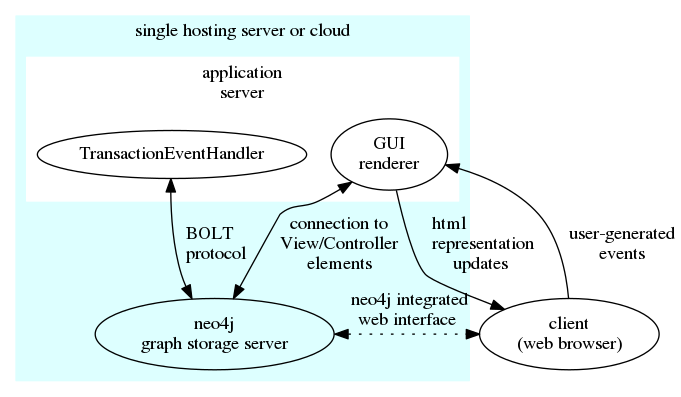
\includegraphics[width=\textwidth]{fig/architecture.png}

\noindent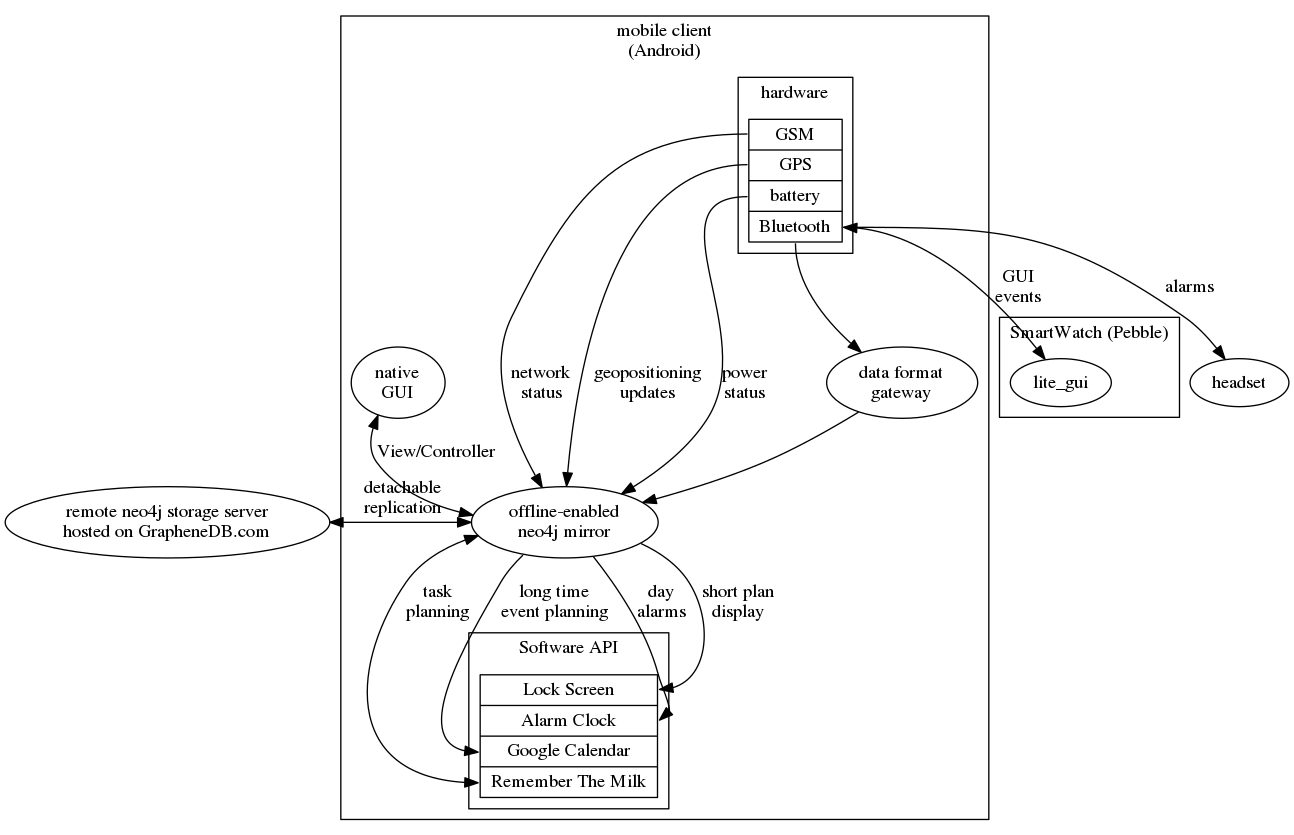
\includegraphics[width=\textwidth]{fig/mobile.png}

\noindent
\includegraphics[width=0.5\textwidth]{fig/person.png}

\begin{thebibliography}{99}
\addcontentsline{toc}{section}{References}
\bibitem{book1} book1
\end{thebibliography}


\end{document}
